La arquitectura propuesta inicialmente para el desarrollo del proyecto, representada en la figura \ref{fig:arqui_prop}, está basada en una arquitectura cliente-servidor, en la que los clientes (dispositivos android) se comunican con un servidor central, encargado de direccionar la petición del usuario al servidor que ofrezca el servicio solicitado. A su vez, se tiene una capa de persistencia donde se llevará registro de la información del sistema y de los usuarios.

\begin{figure}[!htb]
  \begin{center}
    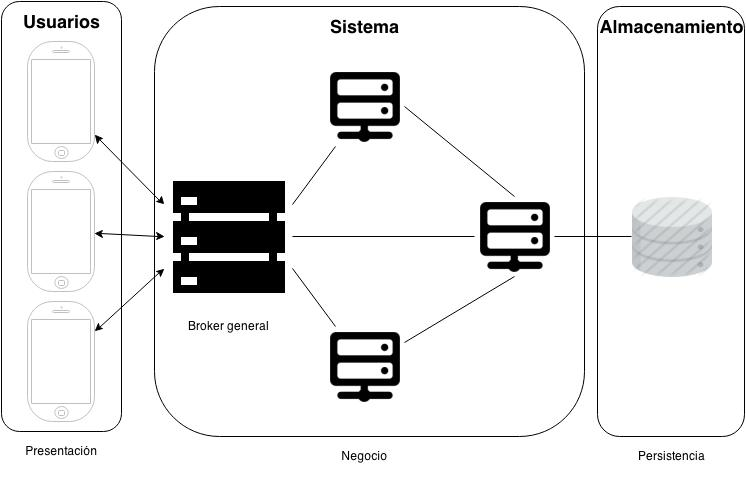
\includegraphics[width=10cm]{./imagenes/arquitectura_propuesta.jpg}
    \caption{Propuesta de arquitectura}
    \label{fig:arqui_prop}
    \textbf{Fuente:} Autores.
  \end{center}
\end{figure}
